

\documentclass[5p,sort&compress]{elsarticle}		
% 5p gir 2 kolonner pr side. 1p gir 1 kolonne pr side.
% Valget sort&compress gjør at referansen [1,2,3] settes som [1-3]. 
% Andre innstillinger for "klassen" elsarticle finnes i dokumentasjonen på CTAN (http://www.ctan.org/pkg/elsarticle)

% Klassen elsarticle er laget for bruk i engelskspråklige tiksskrift. I blokken under bruker vi litt lavnivå TeX-magi for å redefinere bunnteksten på tittelsiden. Ikke bekymre deg for denne biten med kode, det som kommer lengere nede i dokumentet er lettere å forstå!
\makeatletter
\long\def\MaketitleBox{%
  \resetTitleCounters
  \def\baselinestretch{1}%
  \begin{center}%
   \def\baselinestretch{1}%
   \Large\@title\par\vskip18pt
   \normalsize\elsauthors\par\vskip10pt
   \footnotesize\itshape\elsaddress\par\vskip36pt
  \end{center}%
  }
\def\ps@pprintTitle{%
 \let\@oddhead\@empty
 \let\@evenhead\@empty
 \def\@oddfoot{\footnotesize\itshape
       Plan levert til Nikolai	% Bytt ut "Veileder" med navnet på veilederen din!
       \hfill\today}%
 \let\@evenfoot\@oddfoot}
\makeatother

% Encoding for input i tex-filen og encoding for output i pdf-filen
\usepackage[utf8]{inputenc}
\usepackage[T1]{fontenc}
\usepackage{textcomp}

% Last inn en font-pakke. Her bruker vi standard-fonten til LaTeX. 
\usepackage{lmodern}

% LaTeX gjør mye av typografien for deg, blant annet orddeling ved linjeskift og automatisk utfylling av endel tekst. For å kunne gjøre dette må kompilatoren vite hvilket språk dokumentet er skrevet på. 
\usepackage[norsk]{babel}
\usepackage[fixlanguage]{babelbib}

% Mikrotypografiske optimeringer
\usepackage[babel=true]{microtype}

% AMS-utvidelsene for å håndtere matematikk
\usepackage{amsmath}
\usepackage{amssymb}
\usepackage{bm}

% Måltall og enheter er spesielle typografiske dyr som reguleres av strenge regler. For å gjøre det enklere å håndtere tall og enheter på riktig måte bruker vi pakken siunitx.
\usepackage{siunitx}
% Vi tilpasser standardinstillingene til pakken til norske regler. 
\sisetup{
exponent-product = \cdot,
output-decimal-marker  =  {,}, % Pass på å endre desimalskilletegnet til punktum om du skriver på engelsk!
separate-uncertainty = true,
per-mode = symbol,
group-digits = false,
}

% Figurer og tabeller
\usepackage{graphicx} % Denne pakken er standard for å kunne laste inn figurfiler med ulike formater
% Løsne opp på de alt for strenge standardinstillingene for plassering av figurer og tabeller (floats) i LaTeX-kjernen
\renewcommand{\topfraction}{.85}
\renewcommand{\bottomfraction}{.7}
\renewcommand{\textfraction}{.15}
\renewcommand{\floatpagefraction}{.66}
\setcounter{topnumber}{3}
\setcounter{bottomnumber}{2}
\setcounter{totalnumber}{10}
\usepackage{flafter} % For å plassere floats i PDFen første sted LaTeX tillater etter det punktet de er definert i TeX-filen. Om du definerer figuren i TeX-filen rett etter at du refererer til den for første gang vil denne pakken sørge for at de fleste floats havner på greie steder
\usepackage{booktabs} % Denne pakken gir tilgang på endel ekstra kommandoer som legger til rette for god skikk og bruk i tabellformatering.
\usepackage{multirow}
\usepackage[font=small,labelfont=bf]{caption}	% Justering av LaTeX standarder for figurtekst og tabelltekst.

% Hyperreferanser
\usepackage[colorlinks=true,allcolors=blue]{hyperref}
% Noen av navnene for autoreferanser mangler på norsk, så vi ordner opp i det.
\addto\extrasnorsk{%
\def\figureautorefname{figur}%
\def\tableautorefname{tabell}%
\def\sectionautorefname{avsnitt}%
\def\subsectionautorefname{underavsnitt}%
}
% Vi endrer fonten som brukes for URLer til den vanlige tekstfonten.
\urlstyle{same}

%%%%%%%%%%%%%%%%%%%%%%%%%%%%%%%%%%%%%
% Selve dokumentet
%%%%%%%%%%%%%%%%%%%%%%%%%%%%%%%%%%%%%

\begin{document}

% I "front matter" angir vi formalia knyttet til dokumentet -- tittel, forfatter, tilknytning og sammendrag
\begin{frontmatter}

\title{Plan for eksperimentelt prosjekt i fysikk}

% I forfatterlisten legger vi inn "ikke-brytende" mellomrom etter initialene
\author{Andreas A. Mats S. Peter H. Thomas B.}

\end{frontmatter}


\section{Eksperiment}
% Eksperimentdelen skal svare på disse spørsmålene:
% Hvilket/hvilke eksperiment har dere tenkt å gjennomføre? Beskriv kort det fysiske systemet dere har tenkt å se på og hva som er målet med prosjektet. (Hvilke parametere skal bestemmes?) Hvilke fysiske størrelser vil påvirke disse parameterne? (Her trengs det kanskje noen ligninger?) Hvilke størrelser er kjent, og til hvilken nøyaktighet? Hvilke effekter kan du eventuelt neglisjere, og hvorfor? Hvilke størrelser er ukjente og må bestemmes?
Vi skal utføre et eksperiment med dempede svingninger. En stålkule ruller opp og ned i en bueformet bane med konstant krumning. Vi bruker en stålkule fordi den slurer lite og ruller godt i sporet til banen. Ut fra observasjonene og målingene skal vi beregne friksjonskoeffisienten på to ulike måter. Både ved en analytisk- og en eksperimentell løsning hvor vi tar utgangspunkt i en numerisk modell.

I den numeriske løsningen finner vi friksjonskoeffisienten ved å sammenligne de eksperimentelle verdiene med virkeligheten. Når den numeriske løsningen samsvarer med den fysiske bevegelsen vet vi hva friksjonskoeffisienten er.

I den analytiske modellen bruker vi tall fra det fysiske eksperimentet og setter inn i modellen våres. Vi måler endringen i x-posisjon og får ut friksjonskoeffisienten.
Den analytiske modellen tar utgangspunkt i Newtons andre lov.
\begin{equation}
\sum{\vec{F}} = m\vec{a}
\label{eq:Newtons Andre Lov} 
\end{equation}
hvor m er stålkulens masse, og a er akselerasjonen som stålkulen opplever. For å kunne analysere bevegelsen til stålkulen må vi vite hvilke krefter som virker på den. For å gjøre analysen letter vil det være hensiktsmessig å dekomponere kreftene parallelt og normalt på bevegelsesretningen. Stålkulen blir påvirket av kontaktkrefter og fjernkrefter. Tyngdekraften er den eneste fjernkraften og dekomponeres til to komponenter.
\begin{equation}
mg_{p} = mg\cdot\sin(\alpha)
\end{equation}
\begin{equation}
mg_{n} = mg\cdot\cos(\alpha)
\end{equation}

\begin{figure}[tbp] 
\centering
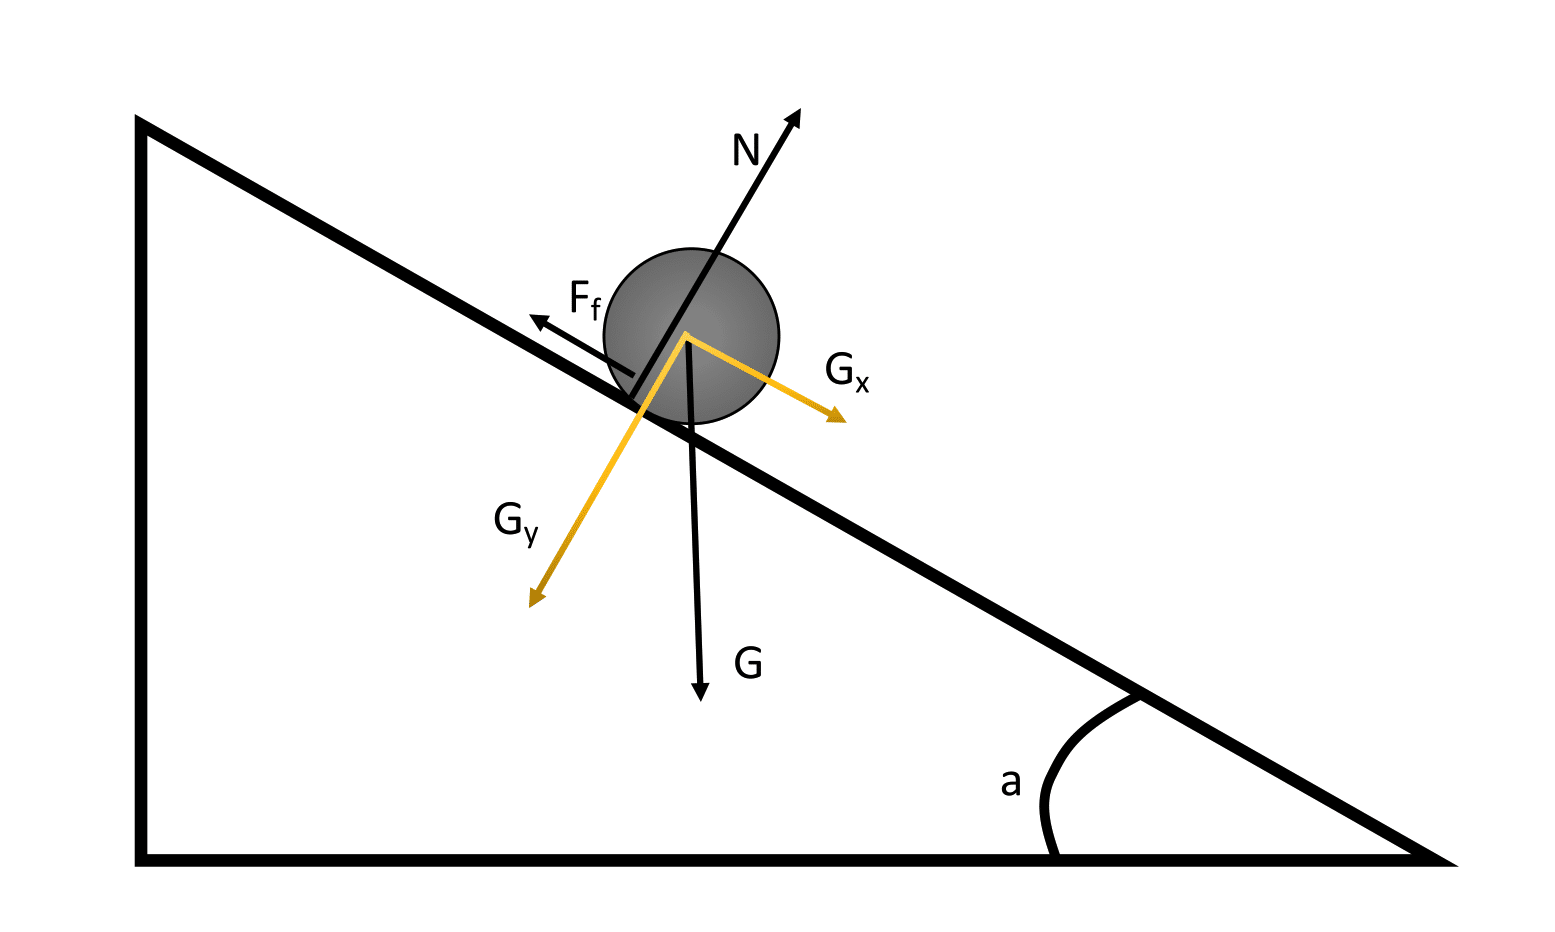
\includegraphics[width=0.4\textwidth]{thomasLOLOLOL.png}

\caption{Krefter som påvirker ballen, dekomponert i x og y retning i henhold i rulleretning.}
\label{fig:pendel} % Som med ligningen er dette det interne navnet på figuren.
\end{figure}

Kontaktkrerftene er normalkraften og friksjonskraften. Vi ser vekk fra luftmotstand i i dette eksperimentet. Vi dekomponerer på tilsvarende måte som med fjernkreftene og får:
\begin{equation}
F_{N} = mg\cdot\cos(\alpha)
\end{equation}
\begin{equation}
F_{F} = \mu\cdot F_{N}
\end{equation}
Der $F_{N}$ er normalkraften rettett oppover med motsatt fortegn av $mg_{N}$ og $F_{F}$ er friksjonskraften i motsatt retning av fartsvektor.
\\
Stålkulens bevegelse kan beskrives som følger.
\begin{equation}
    mgsin\alpha (x) - \ddot{x}\frac{I_{0}}{r^2} - \mu mgcos\alpha (x) \frac{\dot{x}}{|\dot{x}|} = m\ddot{x}
    \label{dynamic}
\end{equation}
Der $I_{0}$ er treghetsmomentet til kula og $r$ er radiusen til kula.
Da får vi.
\begin{equation}
    \ddot{x} = K(sin\alpha (x) - \mu cos\alpha (x) \frac{\dot{x}}{|\dot{x}|}
    \label{diffing}
\end{equation}
Der $K = g/(1+\frac{I_{0}}{mr^2})$
Dersom vi antar at utslaget i vinkelen er så liten at $ \alpha = \sin\alpha $ og $\cos\alpha = 1$  vist i figur 1 og kun ser på bevegelse mot høyre, kan differensiallikningen løses med å finne den homogene løsningen for så å bruke ubestemte koeffisienter metode. Det gir løsningen:
\begin{equation}
x(t) = (-L + K\mu)cos(\sqrt{\omega}t)-K\mu
\end{equation}
hvor $\omega=\frac{K}{R}$\\
Ved å benytte måledataene fra eksperimentet for x posisjonen etter tiden t kan vi løse for friksjonskoeffisienten $\mu$ siden alle andre variabler er kjent ved tid lik en halv periode.

Vi skal også å beregne $\mu$ ved å løse likning \eqref{dynamic} numerisk og sammenligne banen til kulen og numeriske løsninger med ulike $\mu$. 

\begin{figure}[tbp] 
\centering
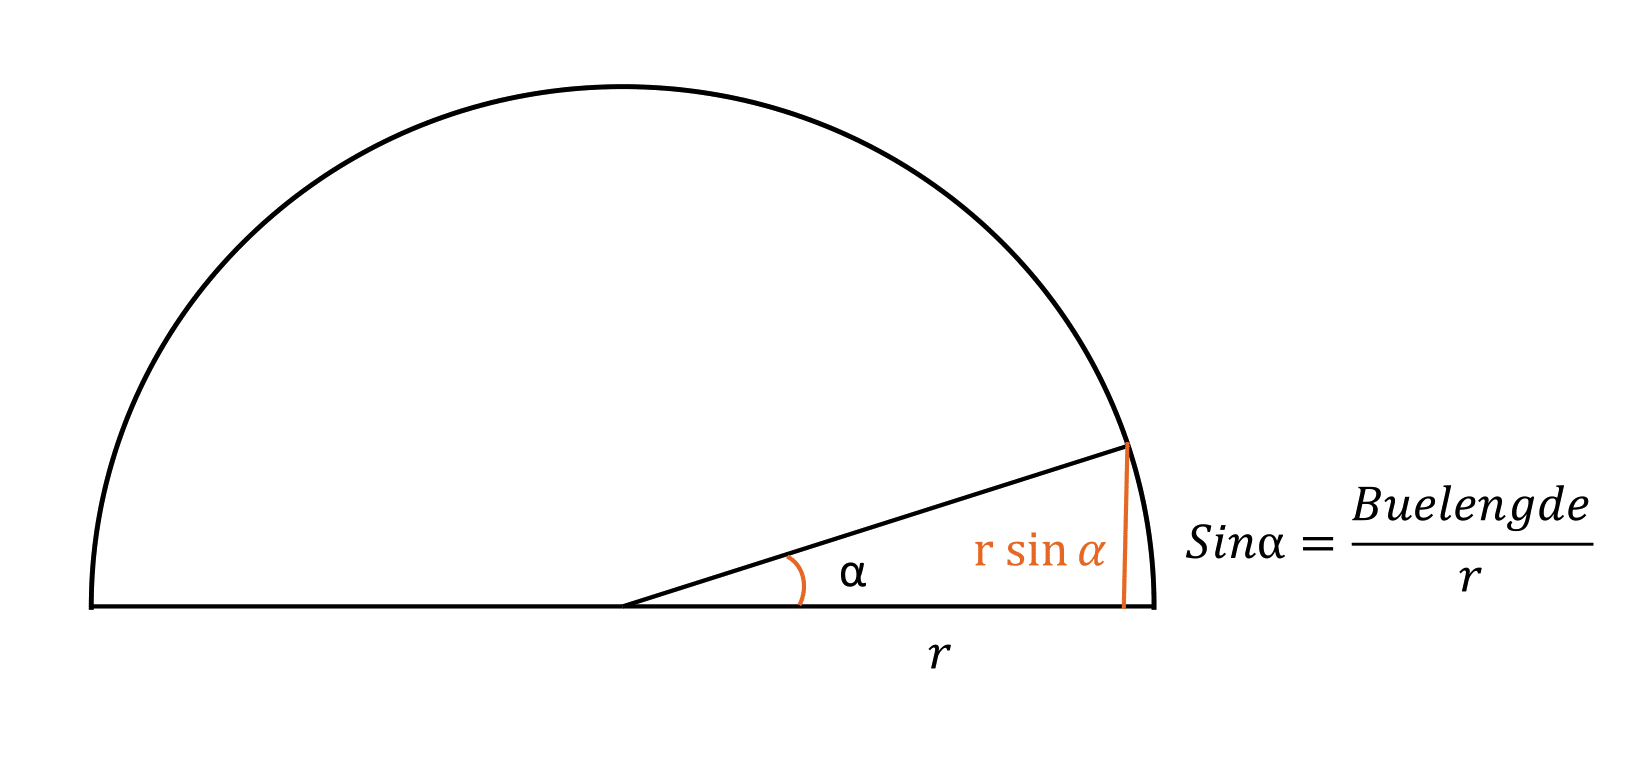
\includegraphics[width=0.4\textwidth]{revidert_halvsirkel_ny.png}

\caption{Representasjon av sinus og cosinus for små vinkler.}
\label{fig:pendel} % Som med ligningen er dette det interne navnet på figuren.
\end{figure}


\section{Praktisk utførelse}
% I den delen av planen som handler om praktisk utførelse skal dere svare på disse spørsmålene:
% Hvordan har dere tenkt å gjennomføre eksperimentet/eksperimentene? Beskriv i detalj hvordan forsøket skal utføres (punktliste). Inkluder en skjematisk figur som viser det eksperimentelle oppsettet og referer til denne figuren i beskrivelsen. Sørg for at forsøket/forsøkene du utfører gir deg mulighet til å bestemme alle de ukjente fysiske størrelsene i systemet. Kan dere utføre noen av målingene på flere måter? Alternative målemetoder kan gjerne brukes til kontrollmåling.

\begin{enumerate}  

\item Setter opp høyhastighetskameraet og Tracker. Stiller det inn med meterstokk og lys, slik som vart gjort på dag én. 
\begin{enumerate}
\item Ordner belysningen, og lyser med en sterk lampe. 
\item Justerer høyhastighetskameraet slik at det peker rett på banen, og sjekker at innstillingene er slik det var lab 1. FF 100fps, eksponering = 0.  
\item Leggee på plass meterstokken under banen, og kalibrerer Tracker til riktig dimensjoner ut i fra meterstokken. Her følges instruksjonene fra dag én på lab om kalibrering av Tracker. 
\end{enumerate}
\item Utfører eksperimentet ti ganger:
\begin{enumerate}
\item Vi starter høyhastighetskameraet og viser først et ark med klippnummer. 
\item Vi slipper så stålkulen fra avmerket punkt og lar det gå gjennom banen fem perioder. 
\item Vi stopper høyhastighetskameraet og repeterer utførelsen.
\end{enumerate}
\item Analyse av dataene i tracker:
\begin{enumerate}
\item Vi definerer stålkulen som objektet Tracker skal følge, og følger det gjennom hele filmen. 
\item Vi finner enderingen i x-posisjonen til stålkulen etter fem fulle perioder og skriver informasjonen inn i en tabell.
\end{enumerate}
\end{enumerate}


\begin{figure}[tbp] 
\centering
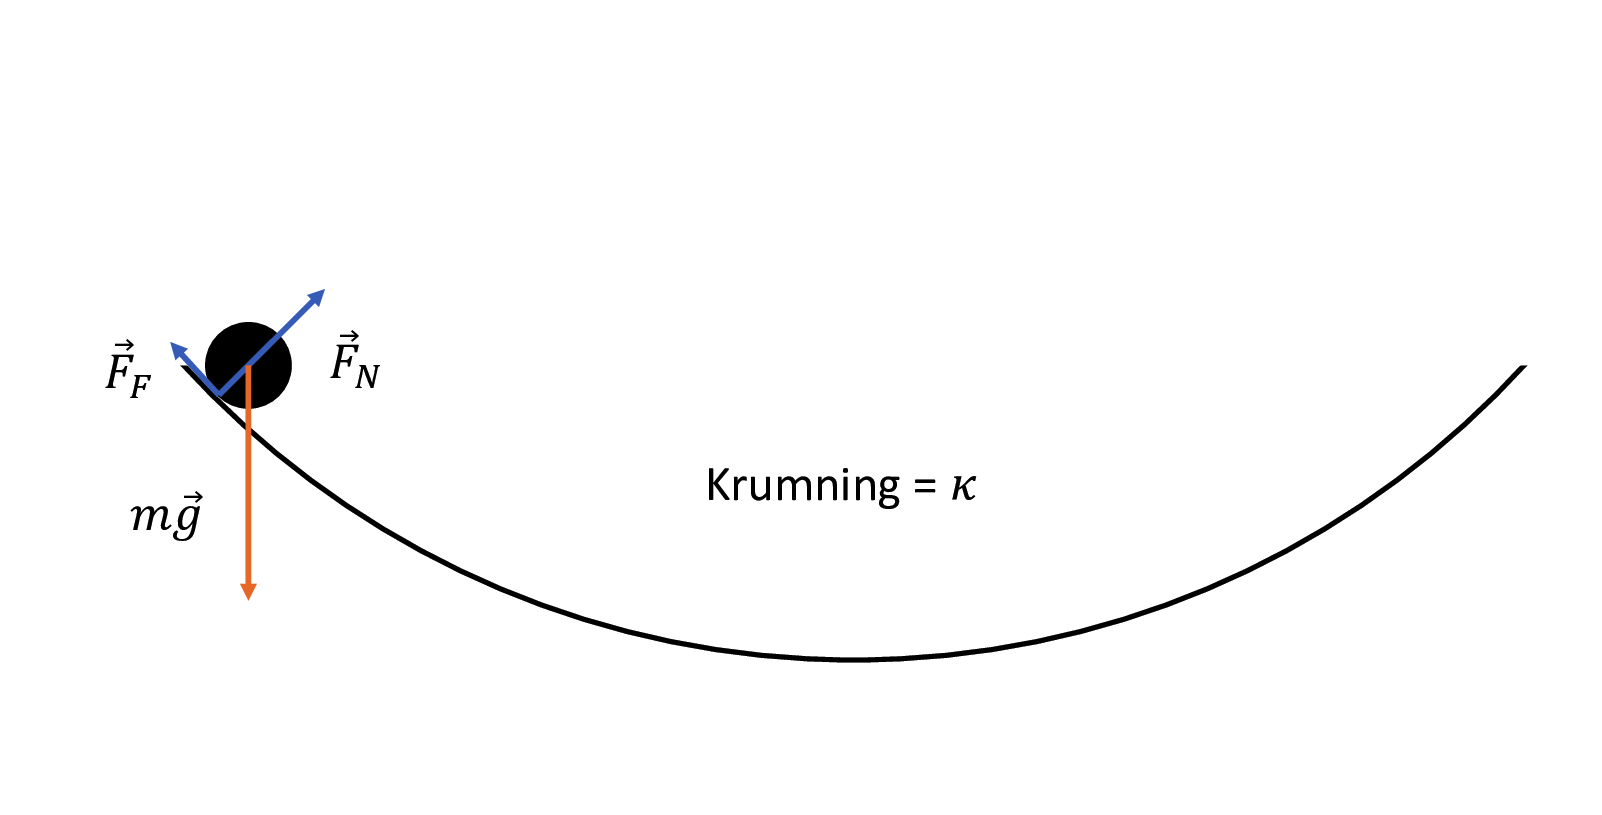
\includegraphics[width=0.4\textwidth]{Figur_til_lab.png}

\caption{Startoppsett av eksperimentet med påvirkende krefter.}
\label{fig:pendel} % Som med ligningen er dette det interne navnet på figuren.
\end{figure}

\section{Usikkerhetsanalyse}
% I behandlingen av usikkerhetsanalysen skal dere svare på disse spørsmålene:
% Hvordan har dere tenkt å bestemme usikkerheten i de ukjente størrelsene? Hvilke feilkilder påvirker disse størrelsene? Finnes det systematiske feilkilder i forsøket deres? Hvilke grep har dere tatt i designet av eksperimentet for å minimere feilene som introduseres?

Det finnes flere mål på usikkerhetanalyse. Vi har blandt annet standardavvik, standardfeil, gjennomsnitt og Gauss' feilforplantningslov.  \\
Gjennomsnittet beregnes ved å legge alle verdiene sammen, for så å dele på det totale antall verdier. \\
Standardavviket er gitt ved å ta kvadratroten av gjennomsnittet av differansen fra gjennomsnittet. Altså gitt ved 

\begin{equation}
s = \sqrt{\frac{1}{N-1}\sum\limits_{i=1}^N(x_{i}-x_{avg})}
\end{equation}
 \\


Standardfeilen er et mål på usikkerheten i gjennomsnittet. Den er gitt ved 
\begin{equation}
\delta x_{avg} = \frac{\delta x}{\sqrt{N}}
\end{equation}

Verdiene vi baserer utregning av friksjonskoeffisienten er lengden $\Delta x$ etter at stålkulen har gått fem perioder i banen.
$\Delta x$ beregnes i tracker med utgangspunkt i meterstokken som er lagt foran startoppsettet. Vi estimerer at feilen til målingen av x posisjonen er på max 5mm. Vi bruker derfor at usikkerheten, $\delta x = \pm $5mm.\\



\subsection{Systematisk feil} 
Når vi skal beregne friksjonskoeffisienten, så antar vi at luftmotstand er lik null. Dette vil føre til avvik i forhold til reell verdi av friskjonen siden det faktisk er en luftmotstand. Størrelsen på denne er ukjent.\\
\vspace{4mm}\\
Disse metodene blir brukt for å beregne usikkerheten til friksjonskoeffesienten vi finner.\\

\section{Numerisk modellering}

Vi tar utgangspunkt i differensiallikningen vi kom frem til tidligere \eqref{dynamic}.
Den andre ordens differensiallikningen kan deles opp til et sett av to første ordens likninger. Innfører $ v = \dot{x}$ slik at settet blir

 \begin{subequations}
    \begin{align}
      \dot{x} = v \\
      \dot{v} = mgsin\alpha (x) - \ddot{x}\frac{I_{0}}{r^2} - \mu mgcos\alpha (x) \frac{\dot{x}}{|\dot{x}|} 
    \end{align}
  \end{subequations}

Denne løser vi ved hjelp av Eulers metode der vi tipper på en $\mu$ som får løsningen x(t) til å samsvare med det fysiske eksperimentet.

\begin{equation}
\vec{y}_{n+1} = \vec{y} + h\vec{f}(t_n,\vec{y}_n)
\label{eq:EulerMethod}
\end{equation}
\\
der $\vec{y}_n = [x_{n} , v_{n}]$ , $ \vec{f}(t_n , \vec{y}_n) = [v_{n} , mgsin\alpha (x) - \ddot{x}\frac{I_{0}}{r^2} - \mu mgcos\alpha (x) \frac{\dot{x}}{|\dot{x}|}]$ og $h$ er steglengden.\\ Eulers metode løses numerisk i matlab.

Den numeriske løsningen av systemet skal brukes til å finne friksjonskoeffisienten ved å sammenligne de teoretiske verdiene med virkeligheten. Når den numeriske løsningen samsvarer med den fysiske bevegelsen vet vi hva friksjonskoeffisienten er.\\

% I numerikkdelen av planen må dere oppgi den fullsteequationndige differensialligningen (Newtons andre lov) som styrer dynamikken til systemet. Beskriv kort hvordan dere har tenkt å løse denne numerisk og hvordan dette skal knyttes til eksperimentet.

\end{document}